\documentclass[14pt]{beamer}


\usepackage{color}
\usepackage{tikz}


\mode<presentation>
{
\usetheme{AlpesLasers}
\setbeamercovered{transparent}
  %\setbeamertemplate{footline}[frame number] 
  %\setbeamertemplate{navigation symbols}{ 
  %\hskip 0.3cm
  %\insertframenumber / \inserttotalframenumber  % <<< frame #
  %\insertpagenumber / \insertpresentationendpage % <<< page #
%} 
}

% font definitions, try \usepackage{ae} instead of the following
% three lines if you don't like this look
\usepackage{listings}
\lstloadlanguages{python}

\usepackage{mathptmx}
\usepackage[scaled=.90]{helvet}
\usepackage{courier}
\usepackage[T1]{fontenc}
\usepackage[english]{babel}
\usepackage[latin1]{inputenc}
\title{Building an efficient simulation framework}
\subtitle{A solution}
\author{St\'ephane Poss}
\date{\today}
% This is only inserted into the PDF information catalog. Can be left
% out.
\subject{PYTHON}

\lstdefinestyle{custompy}{
  belowcaptionskip=1\baselineskip,
  breaklines=true,
  xleftmargin=\parindent,
  language=python,
  showstringspaces=false,
  basicstyle=\footnotesize\ttfamily,
  keywordstyle=\bfseries\color{green!40!black},
  commentstyle=\itshape\color{purple!40!black},
  identifierstyle=\color{blue},
  stringstyle=\color{orange},
}
\lstdefinestyle{customsh}{
  belowcaptionskip=1\baselineskip,
  breaklines=true,
  xleftmargin=\parindent,
  language=bash,
  showstringspaces=false,
  basicstyle=\footnotesize\ttfamily,
  keywordstyle=\bfseries\color{green!40!black},
  commentstyle=\itshape\color{purple!40!black},
  identifierstyle=\color{blue},
  stringstyle=\color{orange},
}
\lstdefinestyle{customcpp}{
  belowcaptionskip=1\baselineskip,
  breaklines=true,
  xleftmargin=\parindent,
  language=C++,
  showstringspaces=false,
  basicstyle=\footnotesize\ttfamily,
  keywordstyle=\bfseries\color{green!40!black},
  commentstyle=\itshape\color{purple!40!black},
  identifierstyle=\color{blue},
  stringstyle=\color{orange},
}

\begin{document}
\begin{frame}[plain]
\titlepage
\end{frame}

\begin{frame}
\tableofcontents
\end{frame}

\section{Situation}
\begin{frame}
\frametitle{Recall}
We had:
\begin{itemize}
\item A program that can be executed indirectly
\item Reproducibility
\item A means to control the I/O
\item A way to store the results
\item User convenience
\end{itemize}
What we need:
\begin{itemize}
\item Run many times similar things
\end{itemize}

\centering

\includegraphics[width=0.5\textwidth]{Dirac_logo_RGB.png}

\end{frame}

\section{DIRAC}
\begin{frame}
\frametitle{DIRAC interware}
\begin{itemize}
\item Provides all components to build ad-hoc grid infrastructures
\pause
\item Interconnects computing resources of different types
\end{itemize}
\pause
\alert{$\Rightarrow$ Interware}
\end{frame}

\begin{frame}
\frametitle{Origins}
\begin{itemize}
\item Designed to handle LHCb data
\item "Fix" problems with grid middlewares
\item Proposed pilot job principle
\item Since 2001, recoded from scratch in 2008
\item Used by many communities
\end{itemize}
Developers in Marseille, Barcelona, CERN, etc.
\end{frame}

\section{WMS}
\begin{frame}
\frametitle{Workload management}
\begin{columns}
\column{0.6\textwidth}
Pilot based Workload Management
\begin{itemize}
\item Pre-job is sent to the resource and runs many jobs
\item High user job efficiency
\item Suitable for heterogeneous resources
\item Application of community policies
\end{itemize}
\column{0.5\textwidth}
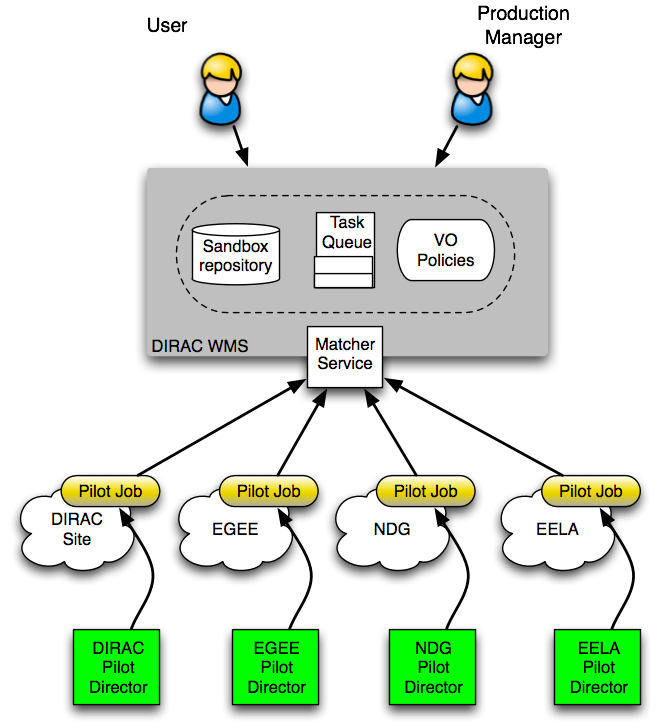
\includegraphics[width=\textwidth]{diracwms.png}
\end{columns}
\end{frame}

\section{Resources}
\begin{frame}
\frametitle{Computing resources}
Grids:
\begin{itemize}
\item EGI, OSG, ARC
\end{itemize}
\pause
Standalone clusters:
\begin{itemize}
\item Local hosts with SSH
\item LSF, BQS, SGE, PBS/Torque, Condor, OAR, SLURM
\end{itemize}
\pause
Clouds:
\begin{itemize}
\item AWS EC2, OCCI, Nova
\end{itemize}
\pause
BOINC
\end{frame}

\section{DataManagement}
\begin{frame}
\frametitle{Data management}
\begin{itemize}
\item Many types of storages supported (SRM, XROOTD, iRods, DAV, DIP, \ldots)
\item Proxy service to unify interfaces
\end{itemize}
Possible to add new ones by extending existing systems
\end{frame}

\begin{frame}
\frametitle{File catalogue}
\begin{itemize}
\item Replica catalogue
\item User metadata catalogue
\item Data provenance
\item Storage reports $\rightarrow$ user storage policies
\item User defined datasets
\end{itemize}
\alert{Central component for modern data analysis systems}
\end{frame}

\section{Workflows}
\begin{frame}
\frametitle{Workflows}
\begin{block}{User driven}
\begin{itemize}
\item User pre-defines all the tasks and their relations
\end{itemize}
\end{block}
\pause
\begin{block}{Data driven}
\begin{itemize}
\item Tasks created when new data available
\item jobs, data replications, etc.
\end{itemize}
\end{block}
\end{frame}

\section{Framework}
\begin{frame}
\frametitle{Framework}
Easy to add components:
\begin{itemize}
\item Everything is PYTHON
\item Extensive documentation
\item Few types: services, agents, UI
\end{itemize}
Multiple interfaces
\begin{itemize}
\item Command line
\item Web portal
\item Python API
\end{itemize}
\alert{Complete middleware for distributed computing systems}
\end{frame}

\section{DIRAC as a service}
\begin{frame}
\frametitle{DIRAC as a service}
Client easy to install
\begin{itemize}
\item extensively documented, part of usual tutorial
\end{itemize}
DIRAC services simple to install, \alert{but}
\begin{itemize}
\item Require dedicated resources
\item Configuration/maintenance need experts
\item Monitoring is tedious/boring
\end{itemize}
\alert{Small communities cannot afford it, but need access to computing resources}
\end{frame}

\begin{frame}
\frametitle{France-grilles DIRAC service}
\begin{itemize}
\item Several univ campuses installations in France
\item Joint effort, hosted by CC/IN2P3 in Lyon
\item Distributed team of admins: 5 participating univ
\item 15 communities: biomed, astronomy, physics, etc.
\item Since May 2012: 30 million jobs, up to 50k jobs in parallel
\end{itemize}

\centering
\url{www.france-grilles.fr}\\

\includegraphics[width=0.4\textwidth]{fg.png}

\end{frame}

\begin{frame}
\frametitle{DIRAC4EGI}
Built from FG-DIRAC experience
\begin{itemize}
\item Joint project of several nation grid initiatives (NGI)
\end{itemize}
Operated by EGI.eu

Maintenance/administration managed by FG
\begin{itemize}
\item Operations
\item User support: documentation, wiki, etc.
\end{itemize}
Distributed teams

\url{http://dirac.egi.eu}
\end{frame}

\section{Conclusions}
\begin{frame}
\frametitle{Conclusions}
DIRAC provides
\begin{itemize}
\item robust general purpose framework for building distributed computing systems
\pause
\item transparent user friendly access to computing and storage resources
\end{itemize}
\pause
Already adopted by several user communities and grid infrastructures as general purpose service

\centering 
\url{http://diracgrid.org}\\

\includegraphics[width=0.5\textwidth]{Dirac_logo_RGB.png}

\end{frame}
\end{document}